%!TEX TS-program = pdflatex
% !BIB program = bibtex
% !TeX encoding = UTF-8
\documentclass[preprint,12pt]{elsarticle}
\biboptions{numbers,sort&compress}

\ifdefined\synctex
  \synctex=1
\fi

\usepackage{amssymb}
\usepackage{amsmath}
\usepackage[a4paper,margin=1in]{geometry}
\usepackage{graphicx}
\usepackage{booktabs}
\usepackage{subcaption}
\usepackage{caption}
\usepackage{float}
\usepackage{placeins}
\usepackage{algorithm}
\usepackage{algpseudocode}
\usepackage{multirow}
\usepackage{longtable}
\usepackage{array}
\usepackage{enumitem}
\usepackage{needspace}
\usepackage[hidelinks]{hyperref}
\hypersetup{pdfauthor={},pdfsubject={},pdfkeywords={}}
\usepackage[T1]{fontenc}
\emergencystretch=2em

\graphicspath{{./}}
\journal{Journal of Manufacturing Processes}

\setcounter{topnumber}{3}
\setcounter{bottomnumber}{2}
\setcounter{totalnumber}{5}
\renewcommand{\topfraction}{0.9}
\renewcommand{\bottomfraction}{0.8}
\renewcommand{\textfraction}{0.07}
\renewcommand{\floatpagefraction}{0.8}
\makeatletter
\setlength{\@fptop}{0pt}
\setlength{\@fpsep}{16pt}
\setlength{\@fpbot}{0pt plus 1fil}
\makeatother

\renewcommand{\algorithmicrequire}{\textbf{Require:}}
\renewcommand{\algorithmicensure}{\textbf{Ensure:}}

\captionsetup[figure]{name=Fig.}
\captionsetup[table]{name=Tab.}

% Numeric Elsevier style does not provide author labels for textual citations.

\clubpenalty=10000
\widowpenalty=10000

% BEGIN shared input: numbers.tex










































% END shared input: numbers.tex
% BEGIN shared input: generated_frozen_macros.tex


% END shared input: generated_frozen_macros.tex
% BEGIN shared input: scaled_numbers.tex



























































% END shared input: scaled_numbers.tex
% Quantitative values are expanded from the verified experiment release.
% BEGIN shared input: v9_formal_binding.tex
% Quantitative artifacts generated from the complete v9 inventory.
% final_comparison SHA256: 22b7c88fd0298f88801ff3a5d5af79488d8f5b75b349330e0e01ce336d2f1725

% END shared input: v9_formal_binding.tex
\begin{document}
\begin{frontmatter}
\title{Reinforcement Learning-Based Computer Numerical Control Motion Planning with Adaptive Preview and Jerk-Constrained Action Projection}
\begin{abstract}
% BEGIN shared input: abstract.tex
Two-step computer numerical control (CNC) motion planning fixes the geometry of computer-aided manufacturing (CAM) tool paths before feedrate scheduling, limiting adjustment within the tolerance band. We propose the Jerk-constrained Neural Numerical Controller (J-NNC), which jointly selects steering, feedrate and Adaptive Preview in a closed loop. The policy is learned through proximal policy optimization and fitting to recorded feasible actions. A kinematic constraint module (KCM) converts these decisions into planar motion satisfying kinematic constraints, allowing trajectory shape and feedrate to be adjusted together. In simulation, the controller completes ordered traversal, braking and rest on the long closed path in 444.153{} s, compared with 445.188{} s for the two-step planner. On the dense path, execution takes 14.819{} s, reducing time by 25.75\% relative to two-step planning and 6.48\% relative to fixed-preview control. The same fitted policy attains the shortest complete times among the feasible comparisons on four selected case-study paths at both 1 and 0.5 ms resolution. These comprise the long and dense paths, the curvature-variation path and the neck contour. The trajectories and motion profiles show turning before the corner, feedrate recovery and sustained near-limit cruising within the one-sided 1.25 mm Euclidean tolerance.

% END shared input: abstract.tex
\end{abstract}
\begin{keyword}
computer numerical control \sep reinforcement learning \sep Adaptive Preview \sep jerk-constrained action projection
\end{keyword}
\end{frontmatter}
\raggedbottom
\section{Introduction}
\label{sec:introduction}
Computer numerical control (CNC) motion planning converts tool paths into executable commands subject to contour and kinematic limits. Conventional two-step planning smooths the geometry and then schedules feedrate along the resulting curve~\citep{Sun2022,Yan2023}. Fixing the geometry restricts how the scheduler can distribute corner transitions within the tolerance band~\citep{Erkorkmaz2001,Lee2011}. At consecutive corners, trajectory curvature and feedrate jointly determine acceleration and jerk.

Geometric smoothing provides explicit control over corner shape and contour error. Sencer et al.~\citep{Sencer2014} optimize quintic B\'ezier corner blends for low curvature and schedule S-curve feed transitions subject to drive acceleration and tangential jerk limits. Other smoothing methods address curvature continuity and axis jerk limits~\citep{Fan2015,Zhang2018}; short segments also require control of overlapping transitions~\citep{Hu2024,Yan2023}. Global fitting and filtering coordinate multiple blocks~\citep{Song2021,Yang2015}. Feedrate methods further address normal jerk, drive and chord-error constraints, using upcoming geometry to regulate motion~\citep{Zhang2021,Wu2022,Tsai2010,Song2020,Zhao2013}. These approaches use upcoming geometry while retaining a predefined geometric construction.

Integrated planning methods coordinate geometric smoothing with the motion constraints. Kinematic corner smoothing and integrated acceleration/deceleration interpolation directly coordinate corner motion~\citep{Tajima2016,Tsai2016}. Related formulations address minimum-time cornering, vibration suppression and driving-force limits~\citep{Duan2016,Sencer2015,LiDriving2017}. For mixed line--arc paths, Li et al.~\citep{Li2023} overlap adjacent segment motions and adjust kinematic parameters using a variable jerk-limited feed profile. Their formulation explicitly constrains resultant acceleration and jerk and controls corner error. Five-axis interpolation also addresses feedrate fluctuation and computational efficiency~\citep{Sun2024}. Here, a learned local rule jointly selects steering, feedrate and guide-target distance.

Li et al.~\citep{Li2020} introduced a Neural Numerical Controller (NNC) trained by deep deterministic policy gradient to generate position commands. Its two outputs are direction-angle and step-length rates, denoted $\theta'_t$ and $l'_t$ in their action definition and accumulated in the command update. The observation includes nine forward rays, whose distances to the tolerance boundaries are capped at $r_{\max}=3\varepsilon_{\mathrm{NNC}}$. Here $\varepsilon_{\mathrm{NNC}}$ denotes that paper's error-constraint parameter. NNC therefore already observes upcoming geometry. Its contour-error-based learning objective and reported per-axis kinematic settings differ from the explicit planar projection used here. J-NNC samples reference geometry at fixed distances and learns the guide-target distance as a separate action. The observation sampling distances remain fixed. The original NNC, our evaluated NNC adaptation and the fixed-preview two-action controller with KCM are distinct controllers in the comparison.

Existing learning-based methods also correct neural-network action requests before execution. OptLayer finds an action close to a network prediction using a differentiable quadratic program with state-dependent linear constraints~\citep{Pham2018}. The present kinematic constraint module (KCM) instead projects a next-velocity request onto intersecting planar disks defined by vector velocity, acceleration and jerk limits. An additional release check verifies that acceleration can then decrease within the limits. The KCM enforces the planar kinematic limits; separate complete-trajectory checks verify contour tolerance and ordered coverage.

The remaining problem is to coordinate local trajectory shaping, feedrate and the guide-target distance while maintaining executable planar motion. We propose the Jerk-constrained Neural Numerical Controller (J-NNC), which jointly selects steering, feedrate and Adaptive Preview from current geometric and kinematic observations. Learning combines proximal policy optimization (PPO)~\citep{Schulman2017PPO} with fitting to recorded feasible actions. The KCM converts the combined request into interpolation commands. Fig.\nobreakspace\ref{fig:comparison_arch} contrasts this framework with two-step planning.

\begin{figure}[htbp]
\centering
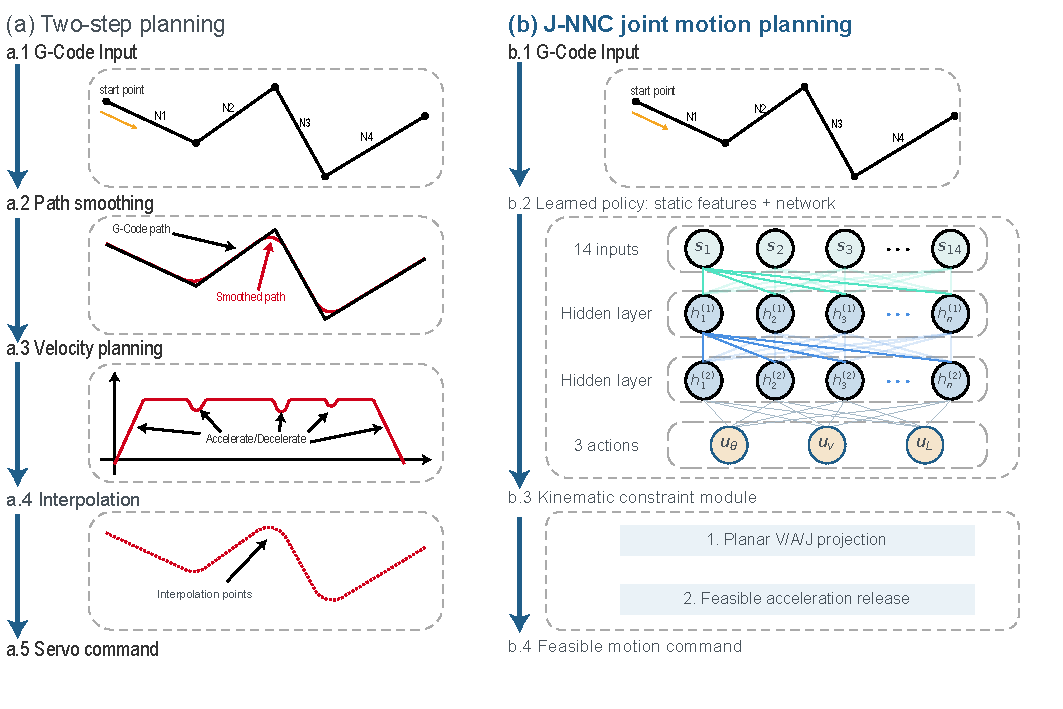
\includegraphics[width=0.9\linewidth]{figure_1.pdf}
\caption{Conventional two-step planning and J-NNC joint motion planning. The policy uses 14 current inputs to select three actions. The KCM converts their combined request into feasible planar motion. In the diagram, $N_i$ labels a path block, $s_i$ is an input component, and $h_i^{(j)}$ is the output of unit $i$ in hidden layer $j$, with $n$ denoting the last unit. The outputs $u_\theta,u_v,u_L$ request steering, feedrate and preview, respectively. V/A/J denotes velocity, acceleration and jerk.}
\label{fig:comparison_arch}
\end{figure}

\begin{samepage}
The main contributions are as follows:
\begin{enumerate}
\item[(1)] A three-action formulation coordinates steering, feedrate and Adaptive Preview within the tolerance band, separating learned guide-target selection from fixed geometric observation sampling.
\item[(2)] A KCM combines projection onto planar velocity disks with checks on subsequent acceleration reduction to enforce velocity, acceleration and jerk limits on the executed commands.
\item[(3)] Complete executions on a long closed path and a corner-dense path compare traversal time and all-corner speed deficit under common contour and motion limits. The evaluation includes ordered coverage, braking and rest.
\end{enumerate}
\end{samepage}

Section 2 defines the planning problem and its constraints. Section 3 presents the method, and Section 4 reports the experimental settings, main results and comparison with fixed-preview control. Section 5 concludes the paper.

% END shared input: introduction.tex
% BEGIN shared input: problem_formulation.tex
\section{Problem Formulation}
\label{sec:problem_formulation}
The planning problem is defined by the reference path, contour tolerance and constraints on the executed motion.

\subsection{Tool Path and Geometric Feasible Region}
Consider a discrete sequence of cutter-location points generated by a CAM system,
\begin{equation}
P_{\mathrm{raw}}=\{p_1,p_2,\dots,p_N\},
\end{equation}
Here $P_{\mathrm{raw}}$ is the reference path, $N$ is the number of cutter-location points, and $p_i\in\mathbb{R}^2$ is point $i$ in the two-dimensional interpolation plane. The prescribed line and arc segments connect these points. Its Cartesian axes are denoted by $X$ and $Y$. Let $\varepsilon$ denote the full width of the contour-tolerance band. Offsetting the reference path by $\varepsilon/2$ on each side defines the geometric feasible region $\Omega$ for a position $x$:
\begin{equation}
\Omega=\{x\mid d(x,P_{\mathrm{raw}})\leq \varepsilon/2\},
\label{eq:feasible_region}
\end{equation}
where $d(x,P_{\mathrm{raw}})$ is the minimum Euclidean distance from $x$ to the finite reference path, including its line and arc segments. The one-sided tolerance is therefore $\varepsilon/2$. Within this band, the controller can adjust the local trajectory to smooth corner transitions while maintaining contour accuracy.

\begin{figure}[htbp]
\centering
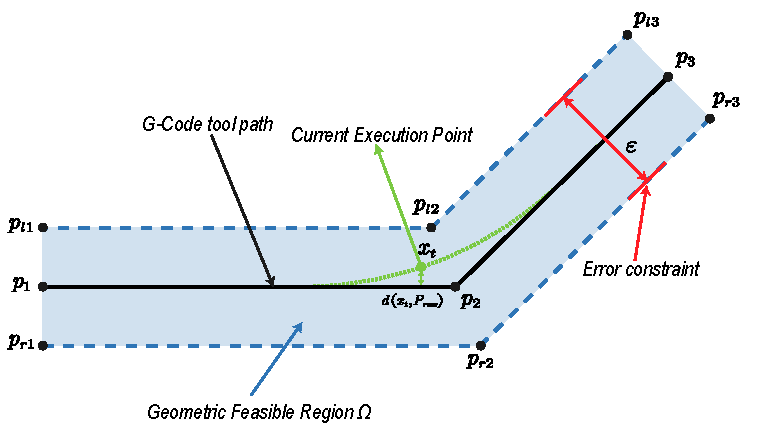
\includegraphics[width=0.9\linewidth]{figure_2.pdf}
\caption{Geometric feasible region formed by the reference path and the contour tolerance band. Points $p_{li}$ and $p_{ri}$ mark the left and right boundaries associated with reference point $p_i$; $x_t$ is the current execution point at decision index $t$.}
\label{fig:feasible_region}
\end{figure}

The reference path is parameterized by arc length for closed-loop control. Tracking variables and forward geometry are extracted at the current projected arc length $\ell_t$ at decision index $t$ to form the observation. An ordered sequence of gates preserves traversal order where different portions of the closed path lie close together.

\subsection{Constrained Action Decision Formulation}
At each decision interval $\Delta t$, the policy receives the current state $s_t$ and returns an action $u_t$. The execution layer converts this request into feasible planar motion at interval $h$. During training, the environment updates the position and motion variables and returns reward $r_t$. For policy $\pi$, discount factor $\gamma\in[0,1]$ and final decision index $H$, the constrained decision problem is
\begin{equation}
\max_{\pi}\ \mathbb{E}_{\pi}\!\left[\sum_{t=0}^{H}\gamma^t r_t\right],
\end{equation}
where $\mathbb{E}_{\pi}$ denotes expectation over trajectories generated by $\pi$. At execution index $k$, the position is $x_k$ and the planar velocity, acceleration and jerk vectors are $v_k,a_k,j_k$. Their magnitude limits are $V_{\max},A_{\max},J_{\max}$, respectively, and $\|\cdot\|_2$ denotes the Euclidean norm. The constraints are $x_k\in\Omega$ and
\begin{equation}
\|v_k\|_2\leq V_{\max},\qquad \|a_k\|_2\leq A_{\max},\qquad \|j_k\|_2\leq J_{\max}.
\end{equation}
These bounds apply to planar vectors and include the acceleration and jerk associated with turning. The motion variables are reconstructed from executed positions as
\begin{equation}
v_k=\frac{x_k-x_{k-1}}{h},\quad a_k=\frac{v_k-v_{k-1}}{h},\quad j_k=\frac{a_k-a_{k-1}}{h}.
\label{eq:physical_differences}
\end{equation}
The initial velocity and acceleration are zero. Derivatives of scalar speed omit changes in direction and cannot fully assess these vector constraints. Heading and curvature describe the resulting trajectory; no separate angular-axis limits are imposed.

A successful execution traverses the entire reference path in order and keeps every command interval within the Euclidean tolerance band. It also completes braking and remains at rest for at least 20 ms. Complete execution time includes startup, traversal, braking and this rest period, so the comparison covers the same complete task.

% END shared input: problem_formulation.tex
% BEGIN shared input: methodology.tex
\section{Methodology}
\label{sec:methodology}
\subsection{Overall Framework}
Adaptive Preview is the preview distance selected by the policy from the current state.

Motion planning for mixed tool paths is formulated as a closed-loop reinforcement learning problem. The policy acts in a path-simulation environment with prescribed contour and kinematic limits. At each decision cycle, the environment constructs the state from tracking error, motion variables and forward geometry. The policy supplies steering, feedrate and Adaptive Preview requests, which the KCM converts into executable planar motion. The executed motion updates the state and provides reward feedback during training.

Fig.\nobreakspace\ref{fig:framework} shows the control loop. Preview selects the forward guide target, steering corrects its direction, and feedrate sets the requested speed. The execution layer constrains the next velocity using the current velocity and acceleration vectors. Evaluation uses the same feedback loop with fixed policy parameters. In the diagram, $f_\theta$ maps the current state $s$ to action $u$, and $\theta$ denotes its fitted parameters. The decoded requests $\alpha,F,L$ are steering correction, feedrate and preview distance. Subscripts are omitted for the held state and action; $v_{k+1}$ is the next executed velocity.

\begin{figure}[htbp]
\centering
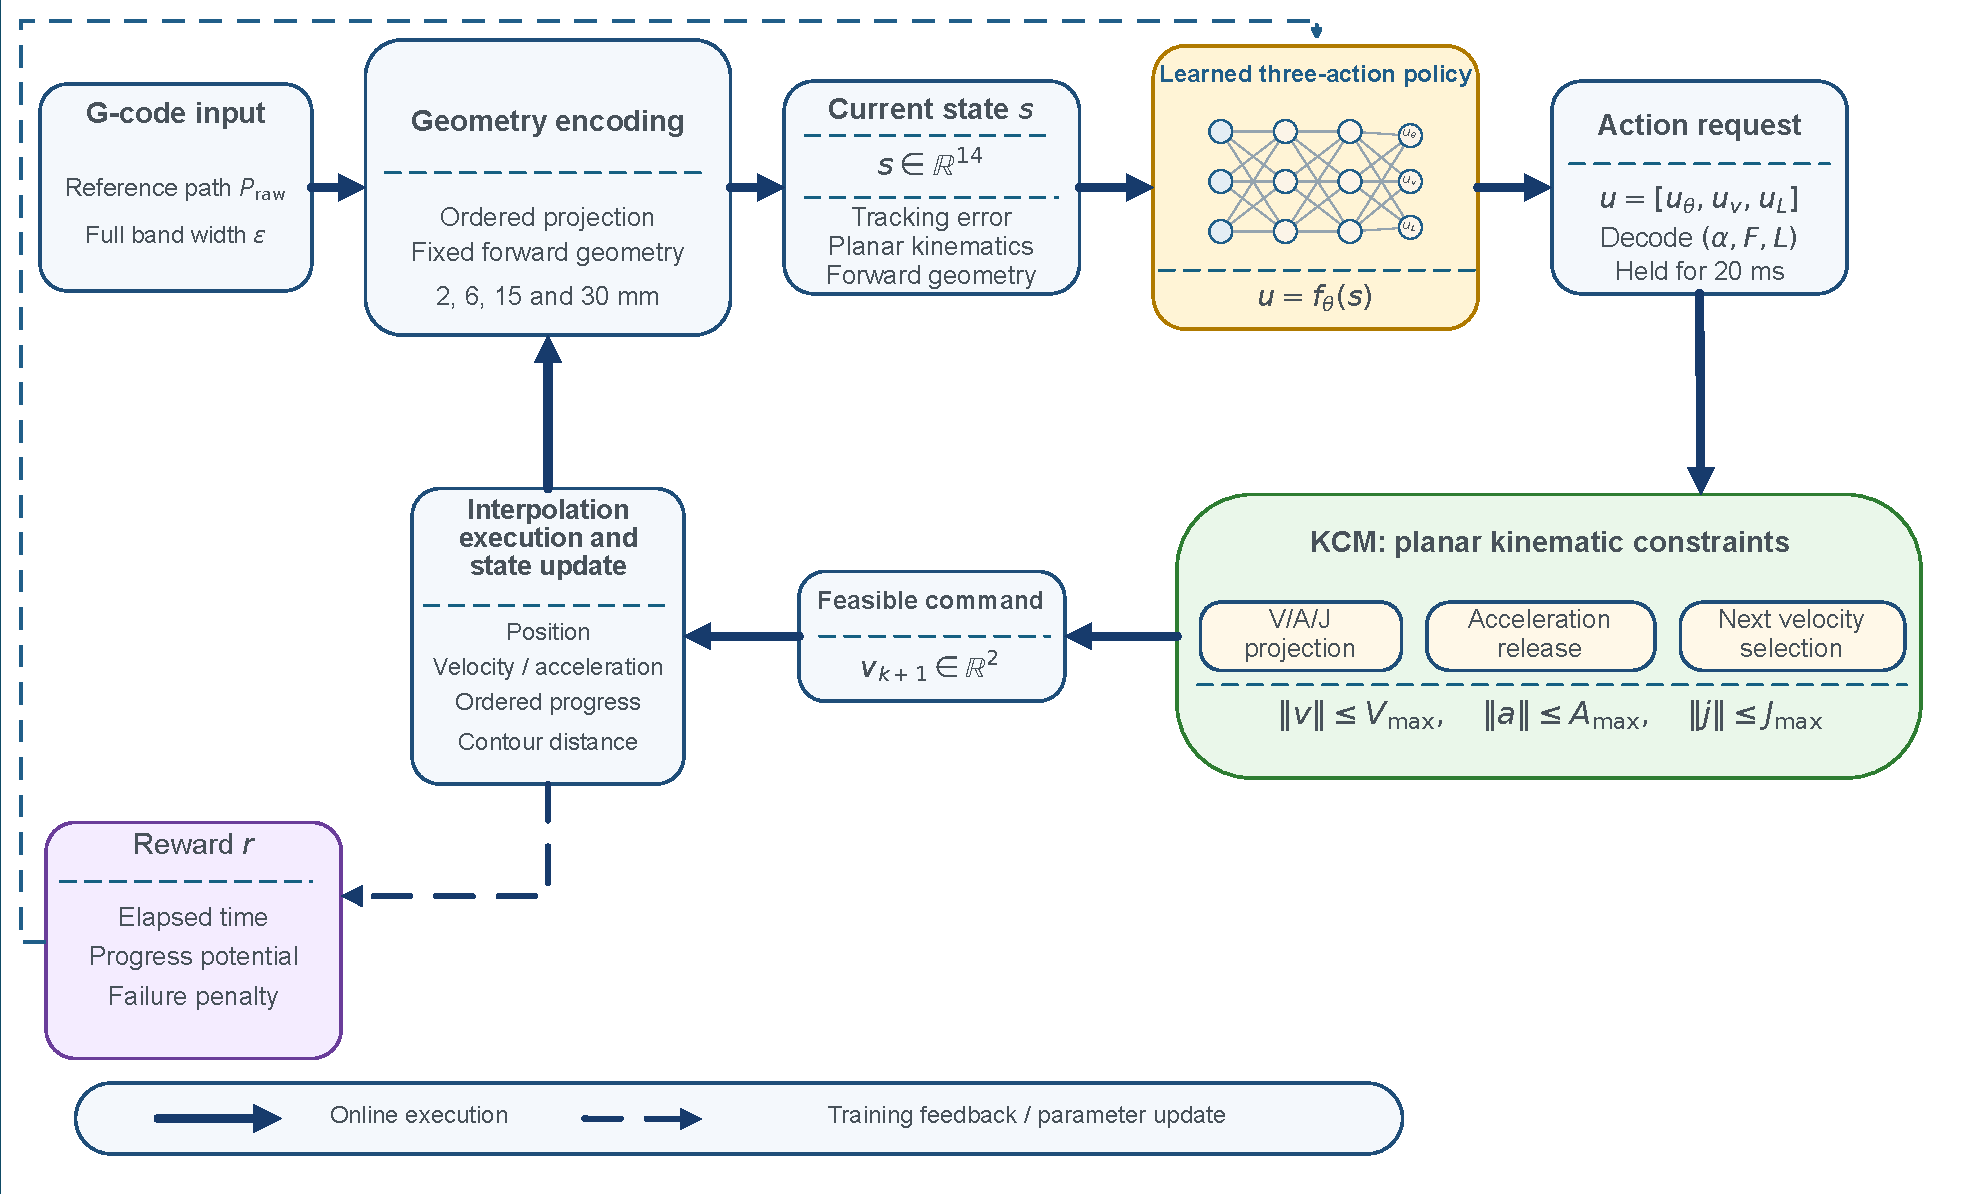
\includegraphics[width=0.9\linewidth]{figure_3.pdf}
\caption{J-NNC control loop. Forward geometry sampled at fixed distances and current motion variables form the 14-dimensional state. The policy outputs steering, feedrate and Adaptive Preview requests, and the KCM determines feasible planar commands. The dashed outer connection represents training feedback and parameter updates.}
\label{fig:framework}
\end{figure}

\subsection{State Design}
The controller uses a 14-dimensional observation of the current state. Tracking and motion variables describe the present motion, while near and far reference points describe upcoming geometry. The columns of $R_h$ are the current heading unit vector and its left normal. Let $t_r,n_r$ denote the local reference unit tangent and unit normal, and let $p(\ell)$ denote a reference point. The current position, velocity and acceleration vectors are $x,v,a$, with time indices omitted. Here $\ell$ is the projected arc length, $d$ is a forward sampling distance, and $\theta_r,\theta_h$ are the reference-tangent and current-heading angles. The input is
\begin{equation}
\begin{split}
s={}&[e_n/1.25,\ R_h^{\mathsf T}v/100,\ R_h^{\mathsf T}a/2000,\ q_{30}^{\parallel},\ \sin(\theta_r-\theta_h),\\
&\{R_h^{\mathsf T}[p(\ell+d)-x]/15\}_{d\in\{2,6,15\}},\ q_{30}^{\perp}],
\end{split}
\label{eq:state14}
\end{equation}
where $e_n=[x-p(\ell)]\cdot n_r$ is the signed normal tracking error. The dimensionless far-reference components $q_{30}^{\parallel}$ and $q_{30}^{\perp}$ are the tangential and normal projections of the displacement to the point 30 mm ahead:
\begin{equation}
q_{30}^{\parallel}=\frac{[p(\ell+30)-p(\ell)]\cdot t_r}{30},\qquad
q_{30}^{\perp}=\frac{[p(\ell+30)-p(\ell)]\cdot n_r}{30}.
\end{equation}
Lengths are expressed in millimeters. The two far-reference components are expressed in the reference frame. Velocity, acceleration and the three near-reference point pairs are expressed in the heading frame. The 14 inputs comprise one tracking error, four kinematic components, one heading sine, six near-point coordinates and two far-reference components.

The near-reference points describe the local transition and recovery, while the 30 mm displacement provides information about geometry farther ahead. These fixed sampling distances are distinct from the preview distance selected by the action. Blending adjacent estimates of reference progress reduces observation jumps at segment boundaries without changing the ordered coverage sequence. The observation excludes elapsed time, global coordinates, corner identifiers, remaining path length and previous actions. The policy stores neither a recurrent state nor an observation history. The static nonlinear features in \ref{app:learning} depend only on these 14 current inputs.

\subsection{Action Space and Kinematic Constraint Module}
At decision $t$, the action $u_t$ contains the normalized steering, feedrate and preview components $u_{\theta,t},u_{v,t},u_{L,t}$, each clipped to $[-1,1]$:
\begin{equation}
u_t=[u_{\theta,t},u_{v,t},u_{L,t}].
\end{equation}
The normalized outputs are mapped to physical requests as
\begin{equation}
\alpha_t=\frac{\pi}{2}u_{\theta,t},\qquad
F_t=50(1+u_{v,t}),\qquad
L_t=6.4+5.6u_{L,t}.
\label{eq:decode}
\end{equation}
Here $\alpha_t$ is a steering correction in radians, $F_t$ is the requested feedrate in mm/s, and $L_t\in[0.8,12]$ mm is the Adaptive Preview distance. The steering action corrects direction rather than commanding angular velocity. The three requests are held for 20 ms, while the guide direction and motion are updated at the smaller integration interval $h$.

The guide direction points from the current position toward the reference point selected by preview distance $L$. Steering corrects this direction, and filtering smooths its changes between interpolation steps. The filtered direction and feedrate $F$ define the desired velocity. Using velocity and acceleration feedback, the execution layer forms a next-velocity request for KCM projection. A release check verifies that acceleration can subsequently decrease within the constraints (\ref{app:kcm}). Contour tolerance and complete ordered coverage are checked separately.

\subsection{Reward Design}
The learning objective combines elapsed execution time, progress shaping and a failure penalty:
\begin{equation}
r_t=-\Delta t_t+\Phi_{t+1}-\Phi_t-\mathbf{1}_{\mathrm{failure}}P_t,
\qquad \Phi_t=\frac{\ell_t-\ell_{\mathrm{total}}}{V_\Phi}.
\label{eq:reward_total}
\end{equation}
Here $\Delta t_t$ is the actual duration of decision step $t$, $\Phi_t$ is a progress potential, $\ell_{\mathrm{total}}$ is total reference length, and $V_\Phi$ scales distance to time. The indicator $\mathbf{1}_{\mathrm{failure}}$ is one on failure and zero otherwise; $P_t$ is the failure penalty. The last PPO training stage uses $V_\Phi=100$ mm/s and zero terminal potential. Failure incurs $P_t=5+\ell_{\mathrm{rem}}/100$ seconds, where $\ell_{\mathrm{rem}}$ is the remaining reference distance in millimeters. For successful undiscounted episodes with the same initial state, the potential differences sum to a constant. Maximizing the return therefore minimizes complete execution time. The learning procedure is described in \ref{app:learning}. Performance is evaluated using executed motion and completion time rather than reward values.

Policy learning combines PPO~\citep{Schulman2017PPO} with fitting to recorded feasible actions. The fixed policy combines a neural network with static features of the same 14 inputs; its complete expression and learning settings appear in \ref{app:learning}.

% END shared input: methodology.tex
\section{Experiments and Results}
\label{sec:experiments}
% BEGIN shared input: experiments.tex
The simulations evaluate joint trajectory shaping and feedrate regulation through complete-path timing, geometric deviation and planar motion profiles.

\subsection{Experimental setup and comparison methods}
All comparisons use complete simulated planar commands, initial rest, and vector limits of 100 mm/s, 2000 mm/s$^2$ and 62\,500 mm/s$^3$. The nominal one-sided tolerance is 1.25 mm. Known arc-to-chord deviation is deducted before evaluating command geometry. Every accepted execution covers the original program in order, keeps each command interval inside the finite-curve corridor, and includes braking and at least 20 ms of final rest. Completion time is assigned only when all these conditions hold.

The reported comparisons comprise four selected complete-path case studies. The long mixed line--arc contour and dense-corner contour in Fig.\nobreakspace\ref{fig:programs} supplied the development trajectories used to train the controller. Two enlarged synthetic programs, described in Section~\ref{sec:additional_paths}, compare the same fitted policy on a curvature-variation path and a neck contour. All four cases use the same tolerance and vector limits.

Policy requests are updated every 20 ms. The heading frame is initialized to the first segment tangent and updated by a 12 ms filter, with its final direction retained during braking. Reference-point queries are clipped to the finite program interval, including for a closed one-lap program.

The learned weights and boundary-search parameters remain fixed throughout evaluation. Deterministic mean actions generate the base plans, followed by finite startup and stopping refinements (\ref{app:boundary}). Both neural controllers receive the same refinement and complete acceptance checks. The statistical unit is one complete program execution; the two resolutions describe its numerical discretization. Timing, geometric deviation, vector kinematics and completion status are computed from the saved final commands.

\begin{figure}[htbp]
\centering
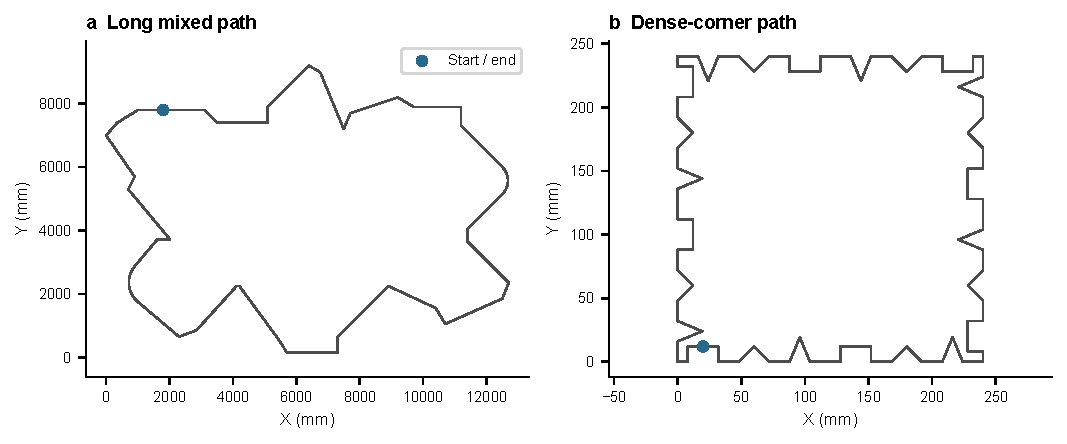
\includegraphics[width=0.98\linewidth]{figure_4.pdf}
\caption{Complete reference programs used for the main comparisons: (a) long mixed line--arc path and (b) dense-corner path. Both programs contribute development records to the learned controller.}
\label{fig:programs}
\end{figure}

% BEGIN shared input: baseline_methods.tex
The comparisons include S2-Q, S2-R, SCMO and COPP, together with fixed-preview control and the NNC adapter.

\label{sec:deterministic_baselines}
The S2-Q comparator separates corner geometry from feed scheduling. Its quintic B\'ezier transitions follow the construction of Sencer et al.~\citep{Sencer2014}; neighboring trims are reduced when they overlap. For turn angle $\varphi$, the control-point ratio is $c/d=(\pi-\varphi)^{0.9927}/2.0769$, and the nominal corner-error parameter is $(1.2447/1.25)\alpha\varepsilon_{\mathrm{poly}}$. Here $\varepsilon_{\mathrm{poly}}$ is the common one-sided polygonal tolerance after subtraction of any certified circular-chord error. The empirical ratio is extrapolated below $30^\circ$; turns above $170^\circ$ and unresolved numerical curvature bounds are rejected. The retained long development program uses its checked original line and arc primitives; the dense program uses its declared polygonal representation. For the enlarged synthetic programs, all deterministic planners use ordered chord merging with a fixed allowance $\delta=0.1\varepsilon_{\mathrm{poly}}$. Replaced vertices lie within this allowance of their merged chord and have monotone projected order. Smoothing uses the remaining budget $\varepsilon_{\mathrm{poly}}-\delta$, and acceptance is checked against the complete original reference and every original gate.

Curve feed is constant within each transition and satisfies
\begin{equation}
v_c\leq\min\left\{V_{\max},\sqrt{\frac{A_i}{\bar\kappa}},\left(\frac{J_i}{\bar g}\right)^{1/3}\right\},
\qquad g=\sqrt{\kappa^4+(d\kappa/ds)^2},
\label{eq:s2_curve_feed}
\end{equation}
where numerical Bernstein enclosures provide the upper bounds with relative tolerance $10^{-3}$, and $A_i=0.999A_{\max}$ and $J_i=0.999J_{\max}$. For the enlarged programs, derivative control vectors are expressed in the local chord-tangent orthonormal frame before applying the same enclosure and scheduling rules. Forward/backward sweeps enforce compatibility between adjacent curve speeds and the intervening straight lengths. S2-Q uses quintic velocity transitions on straight portions, with zero endpoint acceleration and duration
\begin{equation}
T_Q=\max\left\{\frac{15|v_1-v_0|}{8A_i},\sqrt{\frac{10|v_1-v_0|}{\sqrt{3}J_i}}\right\}.
\label{eq:s2_duration}
\end{equation}
This duration is constrained by the chosen polynomial family.

S2-R retains the same geometry and curve-feed bounds but replaces straight scheduling with Ruckig~\citep{Berscheid2021Ruckig}. The unchanged open-source implementation, version 0.12.2, solves each scalar straight-section problem with prescribed position, velocity and zero acceleration at both boundaries. The compatibility sweeps use the corresponding jerk-limited reachability time: $2\sqrt{\Delta v/J_i}$ when $\Delta v\leq A_i^2/J_i$, and $\Delta v/A_i+A_i/J_i$ otherwise. S2-R combines minimum-duration Ruckig timing on the straight subproblems with constant-feed motion on the quintic transitions.

The independent S-curve motion-overlap comparator (SCMO) assigns a rest-to-rest seven-phase scalar motion to each non-collinear block and overlaps neighboring motions subject to a geometric bound. At most two block motions are active. Analytic event states and interior speed extrema determine a common time dilation that enforces the planar vector limits; the geometric allowance also accounts for sampled-command chords. SCMO is constructed for this study from scalar S-curve block motions and the overlap rule described above.

For both S2 variants, $\alpha\in\{1,0.75,0.5\}$ was evaluated on the same two validation programs. All 12 trials completed, and each method selected $\alpha=1$ by maximizing complete runs and then minimizing total completion time. Every deterministic trajectory is independently checked with the same vector limits, command-interval geometry, ordered traversal, initial rest and final-rest requirements as the learned methods.

COPP supplies a second feed-scheduling formulation on the same smoothed geometry. The official version 0.2.3 implementation of TOPP3-SOCP is used with planar vector velocity, acceleration and jerk constraints \citep{Wang2026COPPSoftware}. The path grid uses 0.5 mm spacing on curves and near straight-section endpoints, with 5 mm spacing in the interior of long straight sections. Three sequential convex iterations are specified, with the third supplying the scheduled profile when all iterations succeed. Numerically coincident path stations are merged while retaining derivative constraints from both adjacent pieces. A common time dilation accounts for discretized command kinematics. Its additional 0.1\% reserve is selected on the two validation programs. If command sampling still exceeds a vector limit, the fixed projection rule increases the dilation using the largest speed, square-root acceleration or cube-root jerk ratio across both resolutions, with at most two further projections. Every candidate remains subject to the complete geometric and terminal-state checks. This comparator combines the published open-source scheduler with the common geometry and command evaluator.

The deterministic commands also undergo the same finite startup time-map search in Eq.~\eqref{eq:boundary_time_map}, with their original stopping schedules retained. A shorter prefix is accepted only after the same vector, command-interval and ordered-gate checks; a changed complete trajectory undergoes full acceptance again.

The fixed-preview neural comparator uses a separately trained $14$--$64$--$64$--$2$ policy with 192 local features. Its two action outputs request steering and feedrate, with guide distance held at 3 mm. Both neural controllers use the same vector limits, reference geometry, base execution layer and complete-task criteria. The fixed-preview controller retains its fitted parameters and receives the same startup and stopping searches as J-NNC.

% BEGIN shared input: nnc_method.tex
The NNC comparator is a project adapter using a frozen PPO network with 14 observations and two outputs for angular-velocity and feed requests. Its angular-kinematic feed caps, turn prebraking and endpoint braking remain active. The checkpoint configuration disables the native kinematic projection. The policy is evaluated every 1 ms. At the 0.5 ms command period, each request is held for two commands, with cap-release rates and step-counted durations converted to the same physical time scales. The adapter receives the common reference and effective tolerance and is assessed from initial rest using the same ordered-coverage, command-interval, planar-vector and terminal-rest criteria. Each attempt ends at complete acceptance, the first infeasible command, or its fixed execution budget.

% END shared input: nnc_method.tex

% END shared input: baseline_methods.tex

\subsection{Complete-path performance and motion analysis}
J-NNC completes the long and dense programs in 444.153{} and 14.819{} s under the common conditions (Tab.\nobreakspace\ref{tab:complete_times}). Relative to the traditional two-step schedule S2-Q, the time reductions are 0.23\% and 25.75\%, respectively. With Ruckig used for straight-section scheduling, the reductions are 0.21\% and 24.08\%. The corresponding reductions relative to SCMO are 29.16\% and 20.90\%, and those relative to COPP are 1.15\% and 21.47\%.

% BEGIN shared input: complete_table.tex
\begin{table}[htbp]
\centering
\caption{Complete simulated execution time at 1 ms. Numerical entries satisfy the common geometric and planar vector constraints and include startup, ordered traversal, braking and final rest. A dash denotes an execution that does not satisfy the complete-task criteria.}
\label{tab:complete_times}
\small
\begin{tabular}{lrr}
\toprule
Method & Long path (s) & Dense path (s) \\
\midrule
J-NNC & 444.153 & 14.819 \\
Fixed preview & 444.693 & 15.846 \\
Two-step (S2-Q) & 445.188 & 19.957 \\
Two-step (S2-R) & 445.104 & 19.518 \\
SCMO & 627.017 & 18.735 \\
COPP & 449.333 & 18.871 \\
NNC & -- & -- \\
\bottomrule
\end{tabular}
\end{table}

% END shared input: complete_table.tex

The fixed-preview controller provides a learned comparison with a constant 3 mm guide distance. J-NNC reduces time by 0.12\% on the long program and 6.48\% on the dense program relative to this comparator.

% BEGIN shared input: nnc_results.tex
The project NNC adapter completed 0 of the 4 path--resolution evaluations under the common acceptance criteria. Each attempt reached its first vector-constraint violation at the initial command; the retained prefixes contain 0.5 and 1 ms of executed motion. Completion time is therefore undefined for these attempts, and their constraint peaks refer to the retained prefixes.

% END shared input: nnc_results.tex

The complete trajectories and motion profiles relate these execution times to geometric adjustment and feedrate variation.

Fig.\nobreakspace\ref{fig:trajectory_long} and Fig.\nobreakspace\ref{fig:trajectory_dense} show the complete J-NNC commands and their distances to the finite reference polyline. The maximum command deviations are 1.2219{} mm on the long path and 1.1549{} mm on the dense path. All intervening command segments remain within the common polygonal allowance. The long path contains 2362{} ordered gates, and the dense path contains 84{}; both are traversed completely by the accepted final commands, including their stopping portions.

The long program spends much of its execution near the prescribed speed limit. On the dense program, neighboring transitions occupy a larger fraction of the path. The joint action changes both the direction of the command motion and its requested speed, allowing a corner transition to spread across the available tolerance band. These trajectories are issued position commands in the planar simulator; geometric deviation is measured relative to the reference path.

\begin{figure}[htbp]
\centering
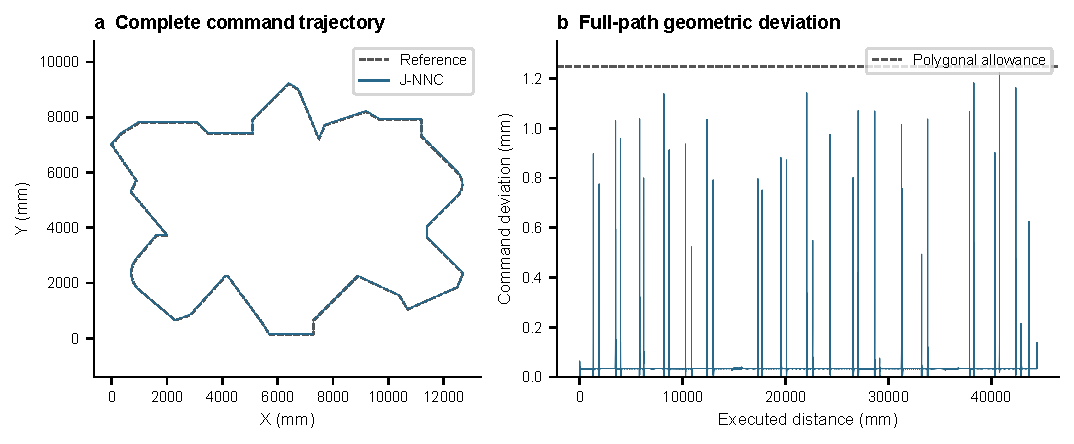
\includegraphics[width=0.98\linewidth]{figure_5.pdf}
\caption{Long-path J-NNC execution: (a) complete command trajectory and (b) command-point distance to the finite reference polyline over the entire executed length. The dashed line in (b) is the polygonal allowance after the arc discretization budget is deducted. Every intervening command segment is checked separately.}
\label{fig:trajectory_long}
\end{figure}
\begin{figure}[htbp]
\centering
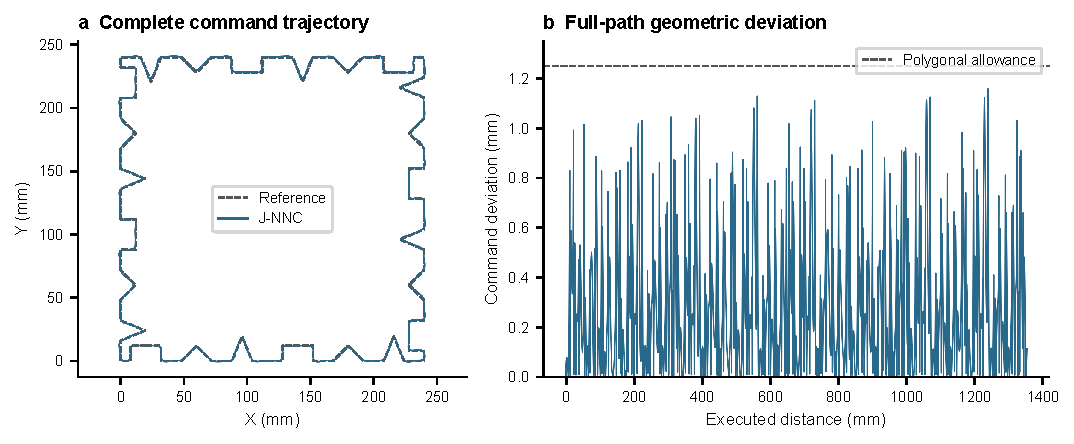
\includegraphics[width=0.98\linewidth]{figure_6.pdf}
\caption{Dense-path J-NNC execution: (a) complete trajectory and (b) geometric deviation over the full executed length. The same controller and complete-execution criteria are used as on the long path.}
\label{fig:trajectory_dense}
\end{figure}

The complete speed, acceleration and jerk profiles in Fig.\nobreakspace\ref{fig:kinematics_long} and Fig.\nobreakspace\ref{fig:kinematics_dense} are reconstructed from the position commands using Eq.~\eqref{eq:physical_differences}. The planar vector norms include the effects of direction changes. J-NNC uses the available acceleration and jerk during local transitions while sustaining a high feedrate between corners.

\begin{figure}[htbp]
\centering
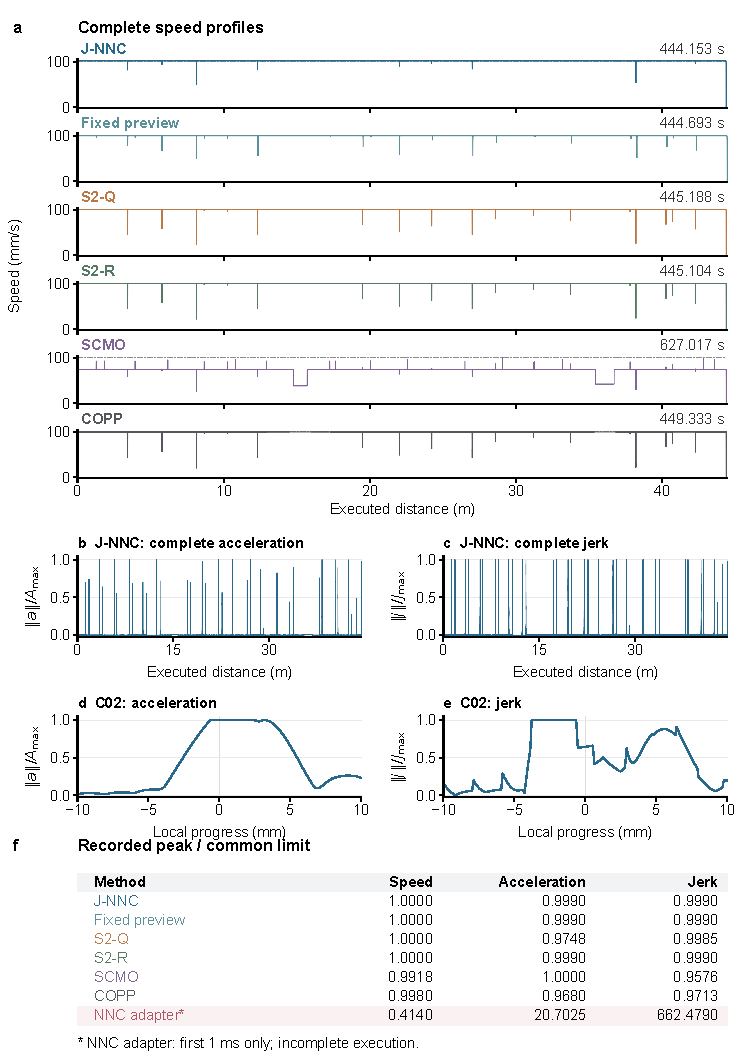
\includegraphics[width=0.98\linewidth,height=180mm,keepaspectratio]{figure_7.pdf}
\caption{Complete simulated command kinematics on the long mixed path at 1 ms. (a) Separate speed profiles on common axes, with complete execution times. (b,c) J-NNC vector acceleration and jerk over the full path. (d,e) Detail at the same C02 window used in Fig.~\ref{fig:main_motion}. (f) Recorded peak-to-limit ratios for all methods. Dashed lines mark the common limits. The NNC adapter entry covers its incomplete first 1 ms.}
\label{fig:kinematics_long}
\end{figure}
\begin{figure}[htbp]
\centering
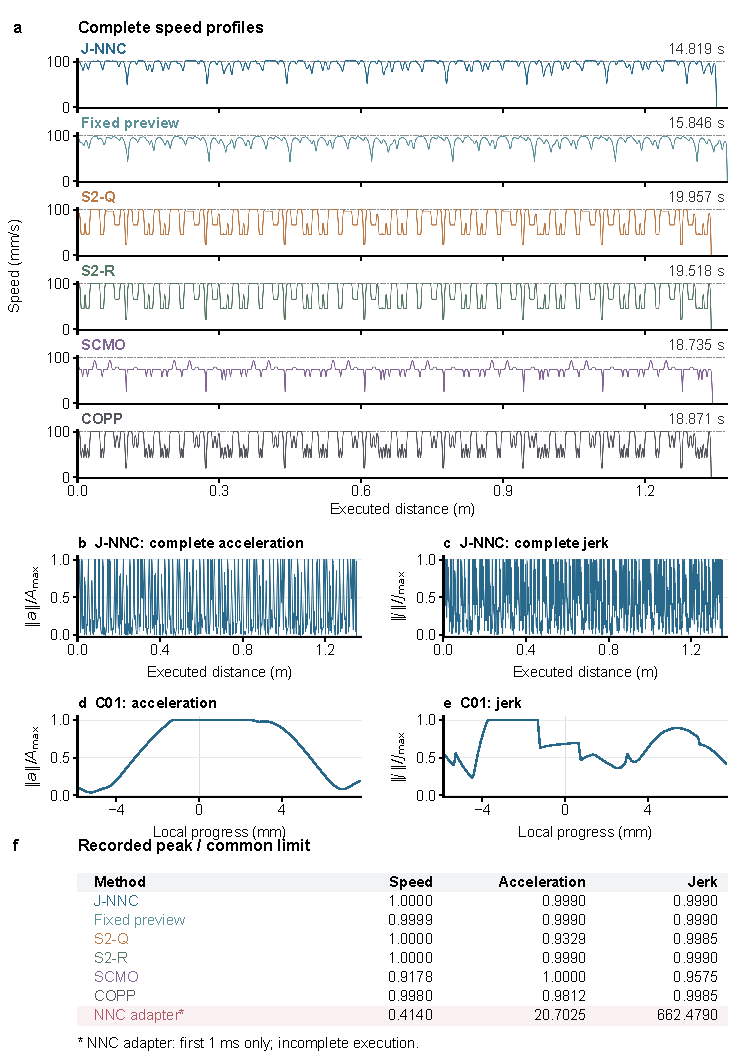
\includegraphics[width=0.98\linewidth,height=180mm,keepaspectratio]{figure_8.pdf}
\caption{Complete simulated command kinematics on the dense path at 1 ms. (a) Separate speed profiles on common axes, with complete execution times. (b,c) J-NNC vector acceleration and jerk over the full path. (d,e) Detail at the same C01 window used in Fig.~\ref{fig:main_motion}. (f) Recorded peak-to-limit ratios for all methods. Dashed lines mark the common limits. The NNC adapter entry covers its incomplete first 1 ms.}
\label{fig:kinematics_dense}
\end{figure}

To relate these profiles to cycle time, define executed length $L_e$ and accumulated speed deficit $D_v$ by
\begin{equation}
L_e=h\sum_k\|v_k\|_2,\qquad
D_v=h\sum_k(V_{\max}-\|v_k\|_2),\qquad
T=\frac{L_e+D_v}{V_{\max}}.
\label{eq:speed_deficit}
\end{equation}
The sums cover every command, including startup, braking and final rest. On the long program, J-NNC executes 44389.68{} mm with a deficit of 25.62{} mm, giving a mean speed of 99.94{} mm/s. On the dense program, the corresponding quantities are 1351.15{} mm, 130.75{} mm and 91.18{} mm/s. The identity separates the contribution of trajectory length from time accumulated below the speed limit.

Fig.\nobreakspace\ref{fig:main_motion} relates local cornering to the full-path deficit. The corners are selected from the reference geometry. J-NNC distributes the turn over a broader transition and maintains a higher speed through the illustrated corners than the two-step schedules. Repeated local deceleration has a larger influence on the dense program, where corner transitions occupy much of the executed motion. On the long path, sustained motion near the speed limit makes the relative time difference smaller. Completion times include the refined startup and stopping portions and the intervening motion.

\begin{figure}[htbp]
\centering
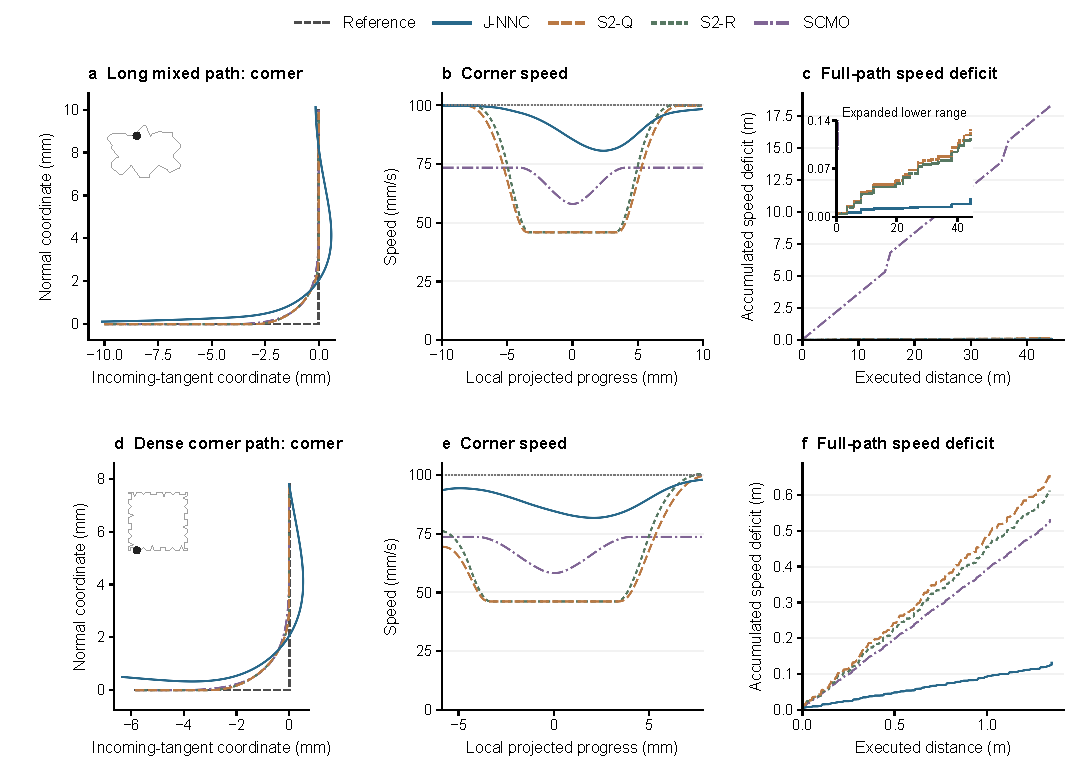
\includegraphics[width=\linewidth]{figure_9.pdf}
\caption{Command motion on the long mixed path (top) and dense-corner path (bottom). Each row shows a local corner with a full-path locator, local speed and accumulated speed deficit over the complete trajectory. The inset in (c) expands the lower range of the same curves. Both J-NNC curves use the final accepted commands, including boundary refinement.}
\label{fig:main_motion}
\end{figure}

\subsection{Cross-path applicability}
\label{sec:additional_paths}
The two selected synthetic cases are tenfold geometric variants of the curvature-coupon and neck-contour programs. Their reference lengths are 909.85{} and 2042.12{} mm, respectively. The coupon contains small, gradually varying turns, whereas the neck contour combines unequal circular lobes and concave transitions. Both neural methods use the same finite boundary refinement for their complete base plans, with unchanged policy weights, nominal tolerance and planar vector limits. Re-discretizing the enlarged circular arcs retains the original chord-error cap, leaving a polygonal allowance of 1.2450{} mm for the neck contour.

With the policy weights fixed, J-NNC completes the additional curvature-variation path and neck contour under the common constraints and achieves shorter complete execution times than the feasible comparators at both resolutions (Tab.\nobreakspace\ref{tab:representative_comparison}). These results demonstrate its applicability across the evaluated path geometries. COPP returns a numerical solver error for both programs, while the NNC adapter ends at its first command violating the vector limits. Neither receives a complete execution time.

% BEGIN shared input: comparison_table.tex
\begin{table}[htbp]
\centering\small
\caption{Complete command times and J-NNC time reductions on the enlarged synthetic paths. Reductions are relative to each comparator at 1 ms. A dash indicates no complete execution or no applicable comparison.}
\label{tab:representative_comparison}
\begin{tabular}{lrrr}
\toprule
Method & 1 ms (s) & 0.5 ms (s) & Reduction (\%) \\
\midrule
\multicolumn{4}{l}{\textit{Curvature-variation path}} \\
\addlinespace[2pt]
J-NNC & 9.202 & 9.1995 & -- \\
Fixed preview & 9.205 & 9.2030 & 0.03 \\
Two-step (S2-Q) & 9.219 & 9.2185 & 0.18 \\
Two-step (S2-R) & 9.205 & 9.2045 & 0.03 \\
SCMO & 11.366 & 11.3645 & 19.04 \\
COPP & -- & -- & -- \\
NNC & -- & -- & -- \\
\midrule
\multicolumn{4}{l}{\textit{Neck contour}} \\
\addlinespace[2pt]
J-NNC & 20.516 & 20.5135 & -- \\
Fixed preview & 20.545 & 20.5430 & 0.14 \\
Two-step (S2-Q) & 21.181 & 21.1805 & 3.14 \\
Two-step (S2-R) & 20.840 & 20.8395 & 1.55 \\
SCMO & 25.893 & 25.8910 & 20.77 \\
COPP & -- & -- & -- \\
NNC & -- & -- & -- \\
\bottomrule
\end{tabular}
\end{table}

% END shared input: comparison_table.tex
% BEGIN shared input: scaled_motion_results.tex
Figure~\ref{fig:scaled_motion} shows the path geometry, separate speed profiles and completion-time differences.

% END shared input: scaled_motion_results.tex

% BEGIN shared input: scaled_figure.tex
\begin{figure}[htbp]
\centering
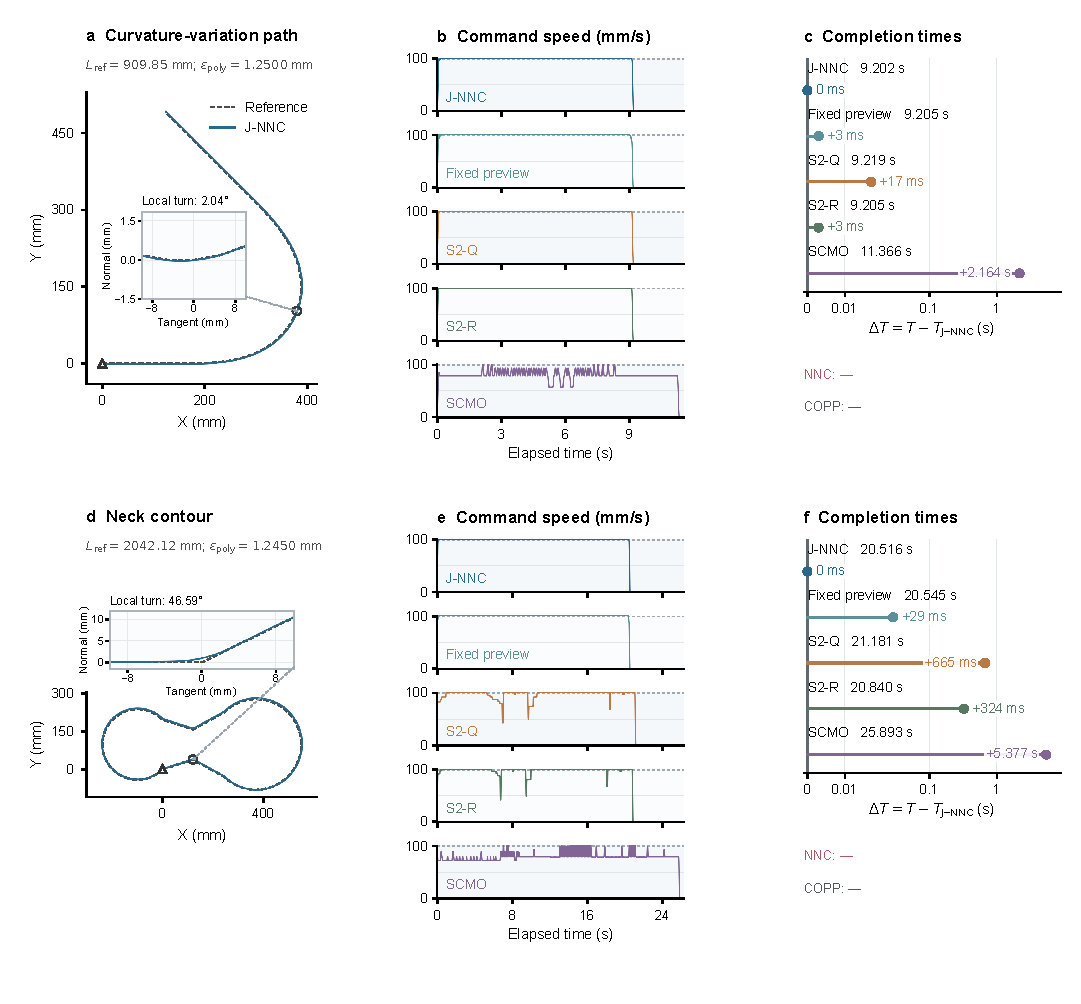
\includegraphics[width=\linewidth]{figure_10.pdf}
\caption{Complete commands on the enlarged curvature-variation path (top) and neck contour (bottom) at 1 ms. Left: full geometry and local tangent/normal views at the first maximum reference turning angle (circles); triangles mark starts. $\varepsilon_{\mathrm{poly}}$ is the effective one-sided polygonal tolerance. Middle: complete command speeds on separate axes with a common scale; dashed lines mark 100 mm/s. Right: completion times and differences from J-NNC. Difference axes are linear to 0.02 s and logarithmic thereafter. Dashes indicate no complete time; NNC denotes the project adapter.}
\label{fig:scaled_motion}
\end{figure}

% END shared input: scaled_figure.tex

\FloatBarrier
\subsection{Temporal resolution and computational cost}
The 1 and 0.5 ms results in Tab.\nobreakspace\ref{tab:resolution} assess numerical sensitivity with the same learned weights and planning parameters, including the 20 ms base-plan policy interval and 12 ms heading filter. Boundary-search durations remain fixed in seconds and use integer multiples of each command period. J-NNC completes the long program in 444.1705{} s and the dense program in 14.8600{} s at the finer resolution. Each paired result includes a complete command-trajectory acceptance check. The finer fixed-preview run of the long program ends before complete traversal and receives no completion time. The larger-scale comparisons in Tab.\nobreakspace\ref{tab:representative_comparison} show a largest time change among paired complete executions of 2.5{} ms.

% BEGIN shared input: resolution_table.tex
\begin{table}[htbp]
\centering
\caption{Time-resolution check with frozen policies and planning parameters. A dash denotes an incomplete execution or an unavailable paired time difference. Each numerical difference compares two complete executions of one program.}
\label{tab:resolution}
\small
\begin{tabular}{llrrr}
\toprule
Program & Method & 1 ms (s) & 0.5 ms (s) & Change (ms) \\
\midrule
Long & J-NNC & 444.153 & 444.1705 & +17.5 \\
Long & Fixed preview & 444.693 & -- & -- \\
Long & Two-step (S2-Q) & 445.188 & 445.1875 & -0.5 \\
Long & Two-step (S2-R) & 445.104 & 445.1035 & -0.5 \\
Long & SCMO & 627.017 & 627.0150 & -2.0 \\
Long & COPP & 449.333 & 449.3325 & -0.5 \\
Long & NNC & -- & -- & -- \\
\midrule
Dense & J-NNC & 14.819 & 14.8600 & +41.0 \\
Dense & Fixed preview & 15.846 & 15.8820 & +36.0 \\
Dense & Two-step (S2-Q) & 19.957 & 19.9565 & -0.5 \\
Dense & Two-step (S2-R) & 19.518 & 19.5180 & +0.0 \\
Dense & SCMO & 18.735 & 18.7335 & -1.5 \\
Dense & COPP & 18.871 & 18.8710 & +0.0 \\
Dense & NNC & -- & -- & -- \\
\bottomrule
\end{tabular}
\end{table}

% END shared input: resolution_table.tex
% BEGIN shared input: cost_results.tex
The recorded training stages, including scheduled evaluations, take 7150.2{} s of wall time. The final action fit takes a further 25.7{} s. These timings exclude earlier teacher-data generation, feature-map discovery and candidate search.

On the enlarged programs, successful deterministic planning takes 5.38{} to 18.20{} s per program for command generation, full-trajectory verification and the common startup search. J-NNC actor evaluation averages 0.45{} to 0.51{} ms per decision on the shared CPU host, excluding geometric and kinematic processing. Boundary refinement and final acceptance take 1.80{} to 11.16{} s. For J-NNC, base-plan generation, refinement and final acceptance together take 7.52{} to 42.48{} s per program in offline computation.

% END shared input: cost_results.tex

% END shared input: experiments.tex
\FloatBarrier
\section{Conclusion}
\label{sec:conclusion}
% BEGIN shared input: conclusion.tex
J-NNC plans CNC motion along mixed reference paths under contour and kinematic constraints. The policy jointly selects steering, feedrate and Adaptive Preview to coordinate trajectory shaping and feedrate regulation. The planar KCM projects the combined request into motion satisfying the velocity, acceleration and jerk limits. The policy uses 14 current geometric and kinematic inputs without stored history.

The same selected model completes the long and dense paths, including ordered traversal, braking and rest, in 444.153{} and 14.819{} s. Dense-path execution time is reduced by 6.48\% relative to fixed-preview control and by 25.75\% relative to two-step planning. The fixed policy also gives shorter complete times on the additional curvature-variation path and neck contour under the common constraints. The local trajectories and V/A/J profiles show turning before the corner, feedrate recovery and sustained near-limit cruising within the tolerance band.

% END shared input: conclusion.tex
\appendix
% BEGIN shared input: appendix_kcm.tex
\section{Kinematic Constraint Module}
\label{app:kcm}
J-NNC and the fixed-preview controller use the same kinematic constraint module and complete-command acceptance rules.

The guide direction uses the reference point selected by preview distance $L$, at the current reference progress. Steering corrects this direction, and a 12 ms heading filter smooths its changes between interpolation steps. The filtered direction and feedrate $F$ define the desired velocity. For filtered heading rate $\omega$, the normal feedforward acceleration is $a_{\mathrm{ff}}=\operatorname{clip}_{A_i}(\omega R_{90}v_{\mathrm{des}})$, where $R_{90}$ rotates a planar vector by $90^\circ$ and $\operatorname{clip}_{A_i}$ limits its magnitude. The requested jerk is $1600(v_{\mathrm{des}}-v)-80(a-a_{\mathrm{ff}})$, with gains in s$^{-2}$ and s$^{-1}$, respectively. Discrete integration gives the next-velocity request for KCM projection. For current velocity $v_k$, acceleration $a_k$ and candidate next velocity $w$, the one-step feasible set is
\begin{equation}
\mathcal C_k=B(0,V_{\max})\cap B(v_k,A_i h)\cap B(v_k+h a_k,J_i h^2),
\label{eq:disks_main}
\end{equation}
where $B(c,r)$ is a closed planar disk and $A_i=0.999A_{\max}$, $J_i=0.999J_{\max}$ provide internal numerical margins. Substitution in Eq.~\eqref{eq:physical_differences} shows that membership enforces the discrete vector limits. Disk projection considers feasible radial projections and pairwise circle intersections, together with degenerate candidates. When requested feed and current speed both reach the nominal speed limit, a preceding branch also considers same-speed turning candidates.

Single-step feasibility is followed by an acceleration-release check. For a candidate state $(v,a)$ with $q=\|a\|_2>0$ and $u=a/q$, a straight release uses
\begin{equation}
a_m=\max(q-mJ_i h,0)u,\qquad
v_{\mathrm{rel}}=v+h\sum_{m=1}^{M}a_m,\qquad
M=\left\lceil\frac{q}{J_i h}\right\rceil.
\label{eq:release_main}
\end{equation}
The acceleration magnitude decreases and each change satisfies the jerk bound. Intermediate velocities lie on the segment from $v$ to $v_{\mathrm{rel}}$, so both endpoints inside the speed disk certify the release. Zero acceleration needs no release.

A second certificate covers constant-speed turning. Consecutive velocities $v-ha$ and $v$ must have equal magnitude $r\in[1,V_{\max}]$ within $10^{-10}$ mm/s. With $B=0.998J_{\max}$, the check requires $q^2/r<B-\eta_J$, where $\eta_J=1$ mm/s$^3$. If $d$ is the signed angular increment, its next value $d'$ keeps the sign and satisfies
\begin{equation}
|d|-|d'|=\min\!\left\{|d|,\frac{h^2}{2r}\left(B-\frac{q^2}{r}\right)\right\}.
\label{eq:turn_release_main}
\end{equation}
The resulting jerk is bounded by $q^2/r+r|d'-d|/h^2\le(B+q^2/r)/2<B<J_i$; angular increments and acceleration magnitudes decrease. Each release step is checked numerically. A request without a release certificate undergoes at most 24 halvings toward a separately verified backup; the search returns that backup if needed. This search provides conditional kinematic continuation during base-plan generation under fixed positive limits, given an available verified backup. Boundary-refined commands are accepted through the complete-trajectory checks described below.

The ordered tracker retains the next unvisited gate and advances only after a directed crossing within its finite channel. Intersecting adjacent channels are admitted only when the complete reference polyline itself witnesses every gate in order; the executing tracker still starts at the first gate. The simulator evaluates geometry after recording each command. The union of finite-reference-segment capsules must cover the whole command segment, and directed gates must be crossed in order. When the remaining reference distance is at most 12 mm, a bounded search tests nonreversing cubic braking trajectories against the vector limits and a 1 mm endpoint-distance condition. Before execution, the complete candidate brake is checked for traversal of every remaining gate and feasibility of every command interval. Each accepted braking command remains subject to the same command-interval corridor check during execution; a violating brake is an unsuccessful run. It is followed by at least 20 ms with speed at most 0.001 mm/s and acceleration at most 0.01 mm/s$^2$. An unsuccessful brake query returns control to the policy. An unverified kinematic backup, geometric violation or timeout ends the run; complete execution time is assigned only after all acceptance conditions are met.


% END shared input: appendix_kcm.tex
% BEGIN shared input: appendix_learning.tex
\section{Policy Representation and Learning Settings}
\label{app:learning}
The policy combines a multilayer perceptron with local corrections in the current observation space. The base network $m_\theta$ has layers $14$--$64$--$64$--$3$ and $\tanh$ hidden activations. Two fixed feature maps contain 96 preview features and 192 joint-action features. For map $b\in\{p,j\}$, the compact-support Wendland feature is
\begin{equation}
\phi_{b,i}(s)=(1-\rho_{b,i})_+^4(4\rho_{b,i}+1),
\qquad
\rho_{b,i}=\frac{1}{r_b}\left\|\frac{s-c_{b,i}}{\sigma_b}\right\|_2,
\quad r_b=1.2,
\label{eq:frozen_wendland}
\end{equation}
where $(z)_+=\max(z,0)$ and division by $\sigma_b$ is componentwise. The centers and feature scales are shared, frozen quantities obtained from development records. \mbox{With $e_3=[0,0,1]^{\mathsf T}$}, the raw mean action is
\begin{equation}
\begin{aligned}
\mu_\theta(s)={}&m_\theta(s)+0.4e_3\tanh\!\left(W_p\phi_p(s)\right)\\
&+G\tanh\!\left(W_j\phi_j(s)\right),\\
G={}&\operatorname{diag}(0.01,0.08,0.4).
\end{aligned}
\label{eq:policy_mean_main}
\end{equation}
The preview correction acts on the third coordinate; the joint correction acts on all three. These maps depend only on the 14 current inputs and introduce no recurrent state. During base-plan generation, each raw coordinate is clipped to $[-1,1]$ before the physical mapping in Eq.~\eqref{eq:decode}. Steering, feedrate and preview requests are held for 20 ms. The guide direction is recomputed at each interpolation step and smoothed by the 12 ms heading filter.

Training alternates action fitting with four PPO stages on the two development programs. The reward uses elapsed command time and reference progress,
\begin{equation}
\begin{split}
r_t={}&-\Delta t_t+\Phi_{t+1}-\Phi_t
-\eta D_t-\mathbf{1}_{\mathrm{failure}}P_t,\\
\Phi_t={}&\frac{\ell_t-\ell_{\mathrm{total}}}{V_*},
\qquad
D_t=\frac{h}{V_*}\sum_{k\in\mathcal I_t}(V_*-\|v_k\|_2)_+,
\end{split}
\label{eq:training_reward_stages}
\end{equation}
where $V_*=100$ mm/s, $h=1$ ms during PPO, and $\mathcal I_t$ contains every executed interpolation step of decision $t$, including its terminal tail. Terminal potential is zero. The two failure penalties are $P_A=T_{\max}+1\,\mathrm{s}+\ell_{\mathrm{rem}}/(20\,\mathrm{mm/s})$ and $P_B=5\,\mathrm{s}+\ell_{\mathrm{rem}}/V_*$, where $T_{\max}=hN_{\max}$ is the episode budget. Table~\ref{tab:frozen_ppo_stages} specifies the shaping terms and retained updates. In the final PPO stage, a successful full episode has return $-T_{\mathrm{base}}+\ell_{\mathrm{total}}/V_*$. Here $T_{\mathrm{base}}$ is the simulated duration before boundary refinement.

\begin{table}[tb]
\centering
\caption{PPO stages in the trained controller. The continuation column gives the fixed update passed to the next stage.}
\label{tab:frozen_ppo_stages}
\begin{tabular}{lcccc}
\hline
Stage & $\eta$ & Failure penalty & Updates & Continuation\\
\hline
Initial action policy & 0 & $P_A$ & 24 & 16\\
Speed-deficit refinement & 1 & $P_A$ & 24 & 24\\
Preview-cue refinement & 1 & $P_B$ & 24 & 24\\
Guided refinement & 0 & $P_B$ & 24 & 24\\
\hline
\end{tabular}
\end{table}

PPO uses diagonal-Gaussian exploration, a separate $14$--$64$--$64$--$1$ critic, an undiscounted return and generalized advantage estimation with $\lambda=0.98$. Each update collects 2,048 decisions. The clipped policy ratio lies in $[0.8,1.2]$; minibatches contain 256 decisions, with six actor epochs and 32 critic epochs. A full-batch KL check limits accepted updates to 0.03. The guided stage additionally fits recorded action targets at visited states. All four stages execute 24 updates, giving 96 executed updates and 196,608 collected decisions; the selected continuation chain inherits 88 updates.

The intervening offline stages fit recorded motion actions and refine the geometric observations before fitting local feature coefficients. Their six iteration budgets are 1,600, 1,800, 12,000, 12,000, 30,000 and 30,000, with fixed continuation at iterations 600, 1,800, 6,000, 12,000, 16,000 and 8,000, respectively. Four ridge fits then determine the local correction coefficients using shared recorded labels and feature maps. The final action fit uses 6,849 frozen records from the two development programs, including trajectories sampled at 1 and 0.5 ms. Adam runs for 12,000 iterations with 256 records from each program per batch. Its learning rate is $2\times10^{-4}$, multiplied by 0.3 after iterations 4,000 and 8,000; the gradient norm is limited to 1. The action loss uses coordinate scales $(0.015,0.15,0.3)$ and treats saturated labels by their clipped-action equivalence. The feature maps remain fixed during this fit. The final 12,000-iteration checkpoint supplies deterministic actions for base-plan generation. Boundary refinement changes neither the fitted weights nor the recorded policy actions.

% END shared input: appendix_learning.tex
% BEGIN shared input: appendix_boundary.tex
\section{Finite Boundary Refinement}
\label{app:boundary}
After a complete base plan has been generated, a common offline stage evaluates shorter startup and stopping sequences. The intervening commands and the fitted policy remain fixed. Candidate durations are integer multiples of the command period $h$, and the same search is applied to both neural controllers.

For startup, let $x_b(t)$ be the not-a-knot cubic interpolant of the first 200 ms of base-plan positions. A candidate saving $\delta\in\{h,2h,\ldots,20\,\mathrm{ms}\}$ defines
\begin{equation}
\begin{aligned}
\tau(t)&=t+\delta b(u),\qquad
b(u)=10u^3-15u^4+6u^5,\\
u&=\operatorname{clip}_{[0,1]}\!\left(\frac{t-20\,\mathrm{ms}}{100\,\mathrm{ms}}\right).
\end{aligned}
\label{eq:boundary_time_map}
\end{equation}
Commands sample $x_b(\tau(t))$ at period $h$ until the original 200 ms joining point. Positions through 20 ms and from 120 ms onward on the new time axis are copied from the corresponding base-plan samples. The joining point and its two predecessor positions are retained exactly, preserving the discrete joining velocity and acceleration. Three successor positions are included when checking jerk across the join. The largest saving satisfying the vector limits, complete-interval geometry and matching ordered-gate state supplies the startup candidate.

Stopping refinement starts from the original terminal position, velocity and acceleration. The velocity direction defines tangential and normal coordinates. Candidate constant-acceleration prefixes range from zero to 30 ms in steps of $h$. Each prefix is followed by a scalar Ruckig velocity stop~\citep{Berscheid2021Ruckig}, with zero terminal speed and acceleration. Its acceleration and jerk limits are $0.98A_{\max}$ and $0.98J_{\max}$. A discrete cubic profile brings the normal velocity and acceleration to zero over the same sampled duration. Candidate positions are reconstructed from the sampled planar velocities. The search retains the original threshold-qualified rest duration and requires nonreversing motion, the vector limits, complete geometric traversal and the 1 mm endpoint condition. The shortest feasible tail is selected only when it shortens the original stopping sequence.

The search applies when a complete base plan separates the original 200 ms joining point and terminal entrance by more than three command periods. Otherwise, the base plan is retained. The assembled trajectory is checked from its initial rest state through every command interval, every ordered gate and final rest. If any acceptance condition fails, the entire original complete plan is retained. A base plan that does not complete remains incomplete. The policy's observation and action records describe base-plan generation; all reported motion metrics use the final accepted command positions.

% END shared input: appendix_boundary.tex


\begingroup
\setlength{\bibsep}{3pt plus 0.3pt}
\interlinepenalty=10000
\bibliographystyle{elsarticle-num}
\bibliography{references}
\endgroup
\end{document}
